\chapter{Função do Receptor}

\section{Introdução}

Nesse trabalho, os dados de eventos incluídos no catálogo do IRIS (\textit{Incorporated Research Institutions for Seismology}) com magnitude maior que 5,5 entre maio de 2011 e dezembro de 2013 foram utilizados. A Figura \ref{mapa_eventos} mostra eventos sísmicos registrados na estação STA08 mostrando a delimitação dos eventos pela distância epicentral, além de mostrar sismos com magnitude maior que 5.5 mb.

O sismômetro registra a velocidade do terreno ao longo das direções Vertical (Z), Norte-Sul (N) e Leste-Oeste (E), chamado sistema ZNE. No entanto, o sinal bruto nas direções ZNE não está alinhado aos eixos de propagação das ondas geradas pelo sismo, logo a resposta em cada componente mostra uma sobreposição de vários tipos de ondas. Com a finalidade de isolar a contribuição de cada onda registrada nos dados, o sistema de coordenadas dos registros são rotacionadas , através do SAC (\textit{Seismic Analysis Code}), para se alinharem com os eixos de propagação das ondas através da seguinte matriz de rotação:

\begin{eqnarray}
 & & \left[ \begin{array}{c} R \\ T \\ Z \end{array} \right] = \begin{bmatrix} \cos \theta & \sin \theta & 0 \\ - \sin \theta & \cos \theta & 0 \\ 0 & 0 & 1 \end{bmatrix} \left[ \begin{array}{c} E \\ N \\ Z \end{array} \right]
\label{rotacao}
\end{eqnarray}

onde E é a componente leste-oeste do sismograma, N a componente norte-sul, Z a componente vertical, R a componente radial, T a componente tangencial e $\theta$ o backazimute, ângulo entre o Norte da estação sismográfica e a linha que une a estação ao evento sísmico.

O resultado da equação \ref{rotacao} discrimina claramente a contribuição de cada componente  no sismograma. A componente N (norte-sul) transforma-se na componente T (transversal) e guarda os registro da onda SH. A resposta da onda SV é resgistrada na componente radial do sismograma, chamada R, como pode ser visualizada na Figura \ref{sismo_radial}.

\begin{figure}[!ht]
\centering
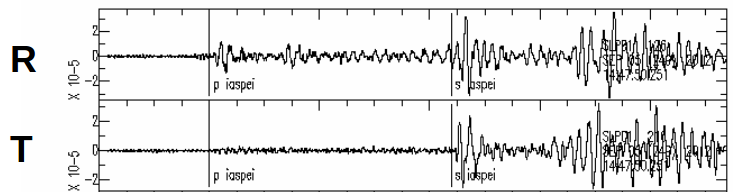
\includegraphics[scale=0.6]{Figs/Componente_Radial_Transversal.png}
\caption{Sismograma mostrando as componentes ENZ e as componentes rotacionadas, Radial e Transversal para a estação estação SLP01, data do evento 05/09/2012, magnitude de 7.59, distância epicentral de $0.01\,^{\circ}$..}
\label{sismo_radial}
\end{figure}

\section{Processamento}

Para o cálculo da espessura crustal na região utilizou-se o método da Função do Receptor, que foi desenvolvido por \cite{Langston_1977}. O programa SAC (\textit{Seismic Analysis Code}) foi usado para fazer o processamento e o cálculo da Função do Receptor. Tal método faz uso do sinal de tele-sismos, geradores de ondas planas de incidência quase-vertical embaixo de uma dada estação. A onda P incide na descontinuidade de Mohorovicic e se decompõe em uma onda P transmitida e uma onda S convertida. A diferença do tempo de chegada das duas ondas, onda S tem velocidade inferior a onda P, e de outras reflexões permite inferir a profundidade da descontinuidade de Mohorovicic, também chamada de Moho, como mostrado na Figura \ref{funcoes_sinteticas} .

\begin{figure}[!ht]
\centering
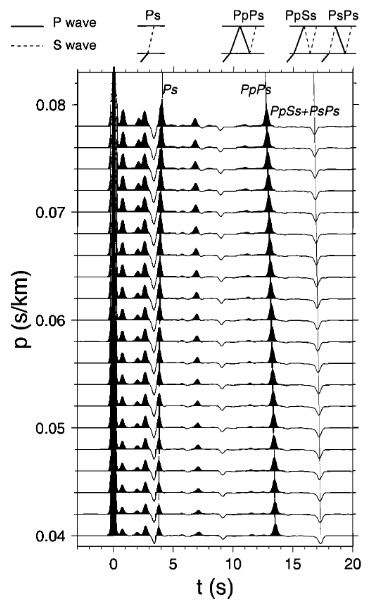
\includegraphics[scale=0.8]{Figs/funcoes_sinteticas.png}
\caption[Funções do Receptor sintéticas em função do parâmetro do raio para o Modelo de Velocidade Padrão do Sul da Califórnia.]{Funções do Receptor em função do parâmetro do raio para o Modelo de Velocidade Padrão do Sul da Califórnia, em \cite{Zhu_Kanamori_2000}. A fase Ps convertida em Moho e suas múltiplas  PpPs, PpSs, e PsPs e seus traços são ilustrados no topo da imagem. Outras reflexões não-rotuladas são as conversões P-S em 5.5 km e 16 km, descontinuidades intracrustais no modelo.}
\label{funcoes_sinteticas}
\end{figure}

Para uma estimativa precisa das Funções do Receptor é essencial que o tempo de chegada da onda P seja determinado com baixa incerteza. Então os dados foram examinados visualmente para registrar o tempo de chegada da onda P direta. 

As Funções do Receptor são calculadas com uma deconvolução da componente radial (R) pela componente vertical (Z), como é mostrado por \cite{clayton_source_1976}, \cite{Langston_1977}, \cite{ammon_isolation_1991}, \cite{cassidy_numerical_1992}, \cite{Zhu_Kanamori_2000}. Essa operação remove efetivamente a resposta instrumental, a assinatura da fonte e a propagação da fonte até a descontinuidade de Moho. O sinal resultante é a assinatura da propagação próxima à estação, então a Função do Receptor é sensível na delimitação da estruturação superficial da crosta embaixo da estação.

Computar as Funções do Receptor é um problema de deconvolução \citep{ligorria_iterative_1999}. \cite{langston_structure_1979} descreve a resposta do deslocamento teórico para uma onda plana P incidindo sobre uma empilhamento de interfaces horizontais ou inclinadas no domínio do tempo pode ser dada por:

\begin{eqnarray} \label{lang_equacao}
D_{V}(t) = I(t) * S(t) * E_{V}(t)
\nonumber
\\
D_{R}(t) = I(t) * S(t) * E_{R}(t)
\\
\nonumber
D_{T}(t) = I(t) * S(t) * E_{T}(t)
\end{eqnarray}

Onde $S(t)$ é a resposta efetiva da fonte em função do tempo de uma onda incidente, $I(t)$ é a resposta do impulso instrumental e $E_{V}(t)$, $E_{R}(t)$ e $E_{T}(t)$ são as respostas do impulso da estruturua vertical, radial e tangencial, respectivamente. A componente $S(t)$ pode ser muito complicada de ser computada, pois ela é relacionada a história do deslocamento no tempo e reverberações na aŕea da fonte.

\cite{langston_structure_1979} assume que eventos profundos observados em dados telessísmicos, na componente vertical do movimento do terreno ($D_{V}(t)$), se comportam como um pulso em função do tempo convoluído com a resposta instrumental e com chegadas tardias menores. Cálculos teóricos para estruturas crustais mostram que reverberações crustais e fases convertidas na componente vertical de ondas P são menores. Então se aproxima:

\begin{eqnarray} \label{lang_suposicao}
I(t) * S(t) \simeq D_{V}(t)
\end{eqnarray}

\cite{langston_structure_1979} faz uma suposição implícita que $D_{V}(t)$ comporta-se como uma função delta de Dirac, como pode ser observado na equação \ref{lang_suposicao}. Assumindo que a resposta instrumental é compensada entre as componentes, $E_{R}(t)$ e $E_{T}(t)$ podem ser encontrados passando para o domínio da frequência a equação \ref{lang_equacao} e fazendo as seguintes deconvoluções:

\begin{eqnarray} \label{lang_resposta}
E_{R}(\omega) =  \frac{D_{R}(\omega)}{I(\omega)S(\omega)} \simeq \frac{D_{R}(\omega)}{D_{V}(\omega)}
\\ \nonumber
E_{T}(\omega) =  \frac{D_{T}(\omega)}{I(\omega)S(\omega)} \simeq \frac{D_{T}(\omega)}{D_{V}(\omega)}
\end{eqnarray}

$E_{R}(\omega)$ e $E_{T}(\omega)$ são retransformadas para o domínio do tempo, importante lembrar que nessa técnica a informação da fase é conservada. A componente radial, $E_{R}(\omega)$ , é chamada de Função do Receptor. \cite{langston_structure_1979} resalta que o resultado da série temporal pode ser interpretado diretamente com um sismograma, permitindo que tempo e amplitude de chegadas possam ser examinadas de uma maneira relativamente inequívoca.

\cite{clayton_source_1976}, \cite{langston_structure_1979}, \cite{ligorria_iterative_1999} mostram que o processo de deconvolução possui um instabilidade numérica devido a vários fatores, como o ruído aleatório contido nos dados e a limitação da banda de frequência. Para acabar com os problemas gerados na deconvolução, \cite{clayton_source_1976} introduz-se um nível de amplitude mínimo permitido da fonte, $c$, nomeado de \textit{water-level}, como pode ser visto na Figura \ref{water_level}. Utiliza-se o \textit{water-level} para reduzir componentes de ruídos espúrios e efeitos de pequenos erros na estimação da localização da fonte. Para evitar a divisão por números pequenos na deconvolução substitui-se os valores pequenos do denominador por uma fração do valor máximo do denominador (para todas as frequências), segundo \cite{Ammon_waterlevel_1997}. Esse método pode agir, em alguns casos, como um filtro "passa-baixa", "passa-alta" e "não-passa", como mostrado na Figura \ref{water_level}. 

Lembrando que a inversa de um número complexo pode ser escrito como $\frac{1}{Z} = \frac{Z^{*}}{ZZ^{*}}$, onde $*$ indica o conjugado complexo, substituindo isto na equação \ref{lang_resposta} teremos:

\begin{eqnarray}
E_{R}(\omega) =  \frac{D_{R}(\omega).D^{*}_{v}(\omega)}{\Phi(\omega)}G(\omega)
\end{eqnarray}

onde:
\begin{eqnarray} \nonumber
\Phi(\omega) = max[D_{v}(\omega)D^{*}_{v}(\omega),cmax{D_{v}(\omega)D^{*}_{v}(\omega)}] 
\end{eqnarray}

e
\begin{eqnarray} \nonumber
G(\omega) = \exp(\frac{-\omega ^{2}}{4a^{2}})
\end{eqnarray}

$G(\omega)$ é um Filtro Gaussiano utilizado para suprimir o ruído de alta frequência na Função do Receptor. Para o fator $a = x$, elimina-se frequências maiores que $x/2$. Logo quanto menor o valor de a, maior é o conteúdo de frequências eliminadas. O parâmetro $a$ do Filtro Gaussiano utilizado varia de acordo com a localização da fonte do evento. Por exemplo, para eventos próximos, $<20º$, o fator $a$ utilizado é  de 15, já para eventos distantes de 2.

\begin{figure}[!ht]
\centering
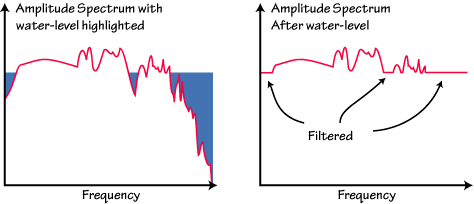
\includegraphics[scale=0.8]{Figs/water_level.png}
\caption{Gráficos mostrando o funcionamento do método \textit{water-level} para a deconvolução no domínio da frequência, segundo \cite{Ammon_waterlevel_1997}.}
\label{water_level}
\end{figure}

No processamento dos dados a deconvolução no domínio do tempo feita é de acordo com a teoria criada por \cite{ligorria_iterative_1999}, esta é nomeada de deconvolução interativa. Tal método segue a ideia de \cite{kikuchi_inversion_1982}, que é usado para estimar funções do tempo de fontes de grandes terremotos. A deconvolução interativa de  \cite{ligorria_iterative_1999} minimiza através do método dos mínimos quadrados a diferença entre o sismograma horizontal observado e um sinal predito pela convolução de um conjunto de picos atualizados interativamente com a componente vertical do sismograma. O cálculo das Funções do Receptor é feito de maneira interativa num conjunto de janelas com diferentes durações. Os melhores resultados são escolhidos de acordo com uma pontuação dada ao ajuste dos dados, a janela que possui a melhor pontuação é escolhida.

\section{Pós-processamento}

Após gerar sismogramas pela deconvolução Interativa, as séries temporais passaram por um processo de triagem para qualificar as que obtiveram melhor resultado. Tal seleção foi feita sob um critério visual, seleção das Funções do Receptor que apresentam um formato  característico mostrado por \citep{langston_structure_1979}, onde o maior pico é a onda $P$ direta e o segundo maior pico é caracterizado pela conversão da onda $P$ em $S$ em Moho. Neste etapa procurou-se excluir Funções do receptor que apresentavam baixo nível sinal-ruído.

Tendo como objetivo a análise da estrutura da crosta, calculou-se a profundidade de Moho, um importante parâmetro, pois é relacionada à geologia e a evolução tectônica regional. \cite{Zhu_Kanamori_2000} propõe um método robusto utilizando a análise das Funções do Receptor para calcular a profundidade de Moho.

Com um modelo da estrutura da Terra, neste caso o modelo IASPEI 91 de \cite{kennet_iaspei_1991}, utiliza-se as velocidades médias na crosta para calcular as diferenças de tempo teórica entre a onda P direta e a onda P convertida em S, bem como os tempos das outras reverberações na crosta. De posse de uma dada velocidade $v_{P}$ ($6.4$ $km/s$), os tempos de chegada podem ser calculados utilizando a profundidade de Moho ($H$), a razão $V_{P}$/$V_{S}$ e o parâmetro do raio ($p$), dependente da localização e da profundidade do evento, e do modelo.

\cite{Zhu_Kanamori_2000} mostra que os tempos teóricos entre $P_{S}$ e $P$ podem ser utilizados para estimar a espessura crustal, dado uma velocidade crustal média:

\begin{eqnarray}
t_{P_{s}} = H.{\sqrt{\frac{1}{V_{s}^{2}} - p^{2}}} - \sqrt{\frac{1}{V_{p}^{2}} - p^{2}}
\end{eqnarray}

\cite{Zhu_Kanamori_2000} demonstra que uma variação de 0.1 na razão $v_{P}$/$v_{S}$ pode acarretar erros de aproximadamente 4 km na espessura crustal. Essa ambiguidade pode ser reduzida utilizando as outras fases, reverberações, da onda P. Tais fases provém informações adicionais, como mostrado nas equações abaixo:

\begin{eqnarray}
t_{P_{p}P_{s}} = H.{{\sqrt{\frac{1}{V_{s}^{2}} - p^{2}}} + \sqrt{\frac{1}{V_{p}^{2}} - p^{2}}}
\end{eqnarray}

\begin{eqnarray}
t_{P_{p}S_{s}+P_{s}P_{s}} = H.{{2\sqrt{\frac{1}{V_{s}^{2}}- p^{2}}}}
\end{eqnarray}

Em situações reais, identificar a conversão $P_{s}$ e as múltiplas é complicado e medir os tempos de chegada em um único traço da função do receptor pode ser muito difícil devido ao ruído de fundo, espalhamento gerado por heterogeneidades crustais e conversões $P_{s}$ de outras descontinuidades de velocidades. Devido a isso, para aumentar a razão sinal-ruído empilha-se as funções do receptor de uma mesma estação. Esse empilhamento é feito no domínio do tempo para um aglomerado de eventos. Para estimar um valor da espessura crustal \cite{Zhu_Kanamori_2000} propõem um empilhamento $H$-$\kappa$ como sendo a função:

\begin{eqnarray} \label{Hk_stack}
s(H,\kappa) = \omega_{1}E_{r}(t_{P_{s}}) + \omega_{2}E_{r}(t_{P_{p}P_{s}}) + \omega_{3}E_{r}(t_{P_{p}S_{s}+P_{s}P_{s}})
\end{eqnarray}

onde $E_{r}$ é a função do receptor (componente radial), os tempos de chegada preditos  $t_{P_{s}}$,  $t_{P_{p}P_{s}}$ e  $t_{P_{p}P_{s}+P_{s}P_{s}}$ correspondente a uma espessura crustal $H$ e a uma razão $V_{p}/V_{s}$ e $\omega_{i}$ são os pesos dos fatores, e $\sum \omega_{i} = 1$, os valores para cada peso pode ser encontrado na Tabela \ref{tabelaMoho} (Anexo 2). 

O método faz uma pesquisa, \textit{grid search}, da espessura crustal, $H$, e da razão $v_{P}$/$v_{S}$, $\kappa$, para calcular o tempo de chegada teórico das ondas P convertidas em S e das múltiplas para cada registro. A melhor combinação de $H$ e $\kappa$, é aquela que maximiza o valor do empilhamento das amplitudes reais das funções receptor, significa que os tempos teóricos são semelhantes aos tempos reais encontrados pela forma da função do receptor.

A incerteza associada a cada um dos parâmetros obtidos pelo método de \cite{Zhu_Kanamori_2000} é estimada pelo método "\textit{bootstrap}", desenvolvido por \cite{efron_statistical_1991}. O método "\textit{bootstrap}" gera do conjunto de Funções do Receptor subconjuntos contendo traços selecionados aleatoriamente. Esse método é repetido para cada subconjunto, resultando num conjunto de parâmetros de $H$ (profundidade de Moho) e de razão $v_{p}/v_{s}$. A média e o desvio padrão dos valores provém um valor médio e uma estimativa da incerteza associada ao cálculo. Não existe uma regra para determinar o número de subconjuntos que precisam ser gerados, o crucial é a busca por um valor que faça a estimativa estabilizar, incluindo as incertezas. Em geral usa-se um valor entre 100 e 200 subconjuntos dependendo da quantidade de traços disponíveis durante o "\textit{bootstrap}".

\cite{assumpcao_crustal_2002},\cite{sand_franca_crustal_2004} e \cite{julia_deep_2008} mostram a necessidade de um cuidado especial ao empilhar as Funções do Receptor, pois existe uma dependência com o ângulo de incidência da onda $P$, acarretando em um deslocamento das reflexões de Moho, isso é observado na Figura \ref{tauptime}. A solução foi a separação das Funções do Receptor de acordo com parâmetro do raio, pois existe uma diminuição no intervalo de tempo entre as ondas $P$ e $P_{s}$ devido o aumento da distância epicentral. Com o aumento da distância epicentral os ângulos de refração se aproximam da vertical, isto diminui a distância entre os pontos de emergência das ondas em Moho. Portanto, o intervalo entre o tempo de chegada destas ondas diminuirá, como pode ser visto na Figura \ref{tauptime}. 

\begin{figure}[!ht]
\centering
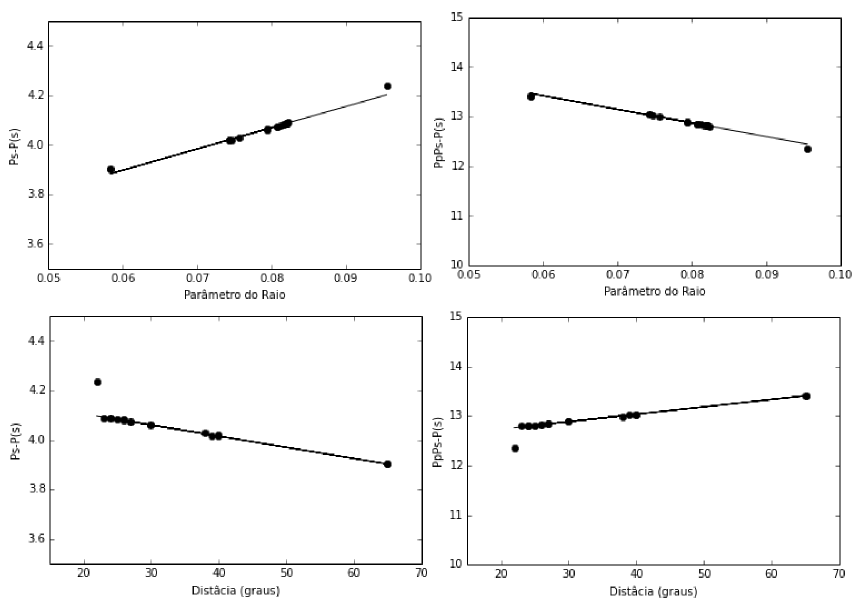
\includegraphics[scale=0.7]{Figs/tempo_teorico_modelo_tauptime.png}
\caption[Tempos teóricos para a reflexão $Ps$ (gráficos à esquerda) e fases $PpPs$ segundo o modelo IASPEI91 de \cite{kennet_iaspei_1991}.]{Tempos teóricos para a reflexão $Ps$ (gráficos à esquerda) e fases $PpPs$ segundo o modelo de \cite{kennet_iaspei_1991}. Os tempos estão classificados segundo o parâmetro do raio e as distâncias epicentrais. Como mostra \cite{sand_franca_crustal_2004} em seu trabalho.}
\label{tauptime}
\end{figure}

Para aumentar a razão sinal-ruído e melhorar a interpretação do arcabouço estrutural da região levou-se em conta a sismicidade ao redor das estações. Visto isso, fez-se uma separação em quatro quadrantes: NE, SE, SW e NW. Cada quadrante representa um agloramedo de eventos, estes aglomerados variam em magnitude e em quantidade, como pode ser observado na Figura \ref{mapa_eventos}. Então as Funções do Receptor para cada estação foi empilhada linearmente para cada grupo de azimute.

Os eventos oriundos da parte nordeste (NE) são escassos e as principais fontes são a Cadeia Meso-atlântica e a cordilheira Alpina na Europa. Já os sismos do sudeste (SE) são originários das Ilhas \textit{South Georgia} e \textit{South Sandwhich}, localizadas no Atlântico Sul, e do Sul da África. A sudoeste é marcante a presença de eventos Andinos, provenientes do Chile e Argentina, e de eventos do Oceano Pacífico. Assim como a sudoeste, os eventos vindos a noroeste (NW) da área são Andinos, oriundo do norte do Chile e do Peru. Também é marcante eventos da América Central, México e Califórnia, estes são bem visíveis na Figura \ref{mapa_eventos}.

O tipo de método utilizado no empilhamento do sinal permite recuperar informações com qualidade e confiabilidade das Funções do Receptor. O empilhamento linear do sinal separado pelo azimute ainda contém um nível de ruído aleatório que não é eliminado pela soma do sinal devido a fatores como a qualidade dos dados, distribuição azimutal dos eventos, \cite{schimmel_noise_1997}. Para isso utilizou-se o Empilhamento Ponderado pela Fase, \textit{Phase Weight Stack (PWS)} , prosposto por \cite{schimmel_noise_1997} como uma ferramenta para reduzir o ruído  incoerente contido no dado, como observado na Figura \ref{empilhamento}-b). Este método concebido por \cite{schimmel_noise_1997} se torna eficiente por conseguir recuperar algumas reflexões coerentes em meio ao ruído, mesmo apresentando uma alteração na forma do sinal. 

Com a finalidade de suprimir este ruído que não é coerente, utiliza-se o empilhamento da fase do sinal como uma medida de coerência para a soma dos traços sísmicos. A ideia consiste em usar o empilhameto da fase como um peso dependente do tempo do empilhamento linear do sinal sísmico. Isto é facilmente realizado pela multiplicação dos empilhamento da fase com o empilhamento linear do sinal, como observa-se na equação \ref{PWS}.

\begin{equation}
\label{PWS}
g(t) = \frac{1}{N} \sum_{j=1}^{N}s_{j}(t)\left | \frac{1}{N} \sum_{k=1}^{N}exp\left [ i\Phi _{k}(t) \right ]  \right |^{v}
\end{equation}

onde $N$ é o número de traços, $s(t)$ o traço sísmico, $\Phi (t)$ a fase e $v$ a potência. 


Segundo \cite{schimmel_noise_1997} cada amostra do empilhamento linear será ponderado pela coerência de suas fases instantâneas. O empilhamento da fase funciona como um filtro com uma certa nitidez da transição entre a semelhança e dessemelhança da fase, que é controlado pela potência $v$. 

Essa dissertação incrementa a metodologia idealizada por \cite{schimmel_noise_1997} visando realçar as múltiplas de Moho que estão indistinguíveis devido o alto nível ruído em algumas Funções do Receptor. \cite{harris_use_1978} cita que janelas são funções ponderadas aplicadas aos dados para reduzir o vazamento espectral associados com intervalos observados finitos, logo o janelamento minimiza as margens de transição em formas de onda truncadas. \cite{andrade_soares_2007} mostra que aplicar uma janela a um sinal no domínio do tempo é equivalente a multiplicar o sinal pela função
que representa a janela. Devido a multiplicação no domínio do tempo ser equivalente à convolução no domínio da freqüência, o espectro de um sinal
janelado é a convolução do espectro do sinal original com o espectro da janela. Dessa maneira, o janelamento modifica a forma do sinal tanto no domínio do tempo quanto no da freqüência.

Os traços das Funções do Receptor utilizados para calcular a fase do sinal foram multiplicado por uma janela Triangular previamente. \cite{harris_use_1978} mostra que a performance da transformada discreta de Fourier em dados janelados é mais eficiente. Com este janelamento prévio, o empilhamento ponderado pela fase (PWS) consegue, além de reduzir o ruído incoerente, recuperar as outras reflexões que não eram bem observadas no resultado gerado pelo PWS, como pode ser observado na Figura \ref{PWS}-c), devido à mistura entre o ruído e o  qualidade das funções do receptor.

\begin{figure}[!ht]
\centering
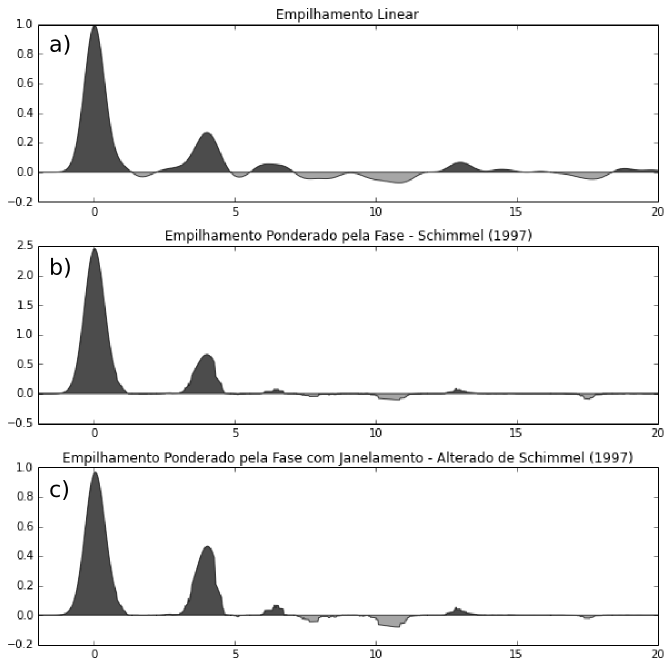
\includegraphics[scale=0.8]{Figs/empilhamento.png}
\caption[Comparação entre os tipos de empilhamento utilizados nas Funções do Receptor.]{Comparação entre os tipos de empilhamento utilizados nas Funções do Receptor. a) Empilhamento linear das funções do receptor separadas pelo azimute na estação SLP01. b)  Empilhamento das funções do receptor ponderado pela fase proposto por \cite{schimmel_noise_1997}. c) Empilhamento das funções do receptor ponderado pela fase com janelamento do sinal}
\label{empilhamento}
\end{figure}

\section{Modelagem das Funções do Receptor}

A modelagem das Funções do Receptor mostra-se uma boa opção para compreender melhor o objeto em estudo. Inicialmente testou-se modelos de velocidade com camadas horizontais baseados aos modelos encontrados na literatura sobre região. Após esta etapa fez-se testes com uma descontinuidade de velocidade inclinada, coerente com uma Moho inclinada mostrada em trabalhos de \cite{sand_franca_crustal_2004}, \cite{flora_solon_ancient_2013} e \cite{Silva_2014} . 

\subsection{Modelos de velocidade para camadas horizontais}

\begin{figure}[!ht]
\centering
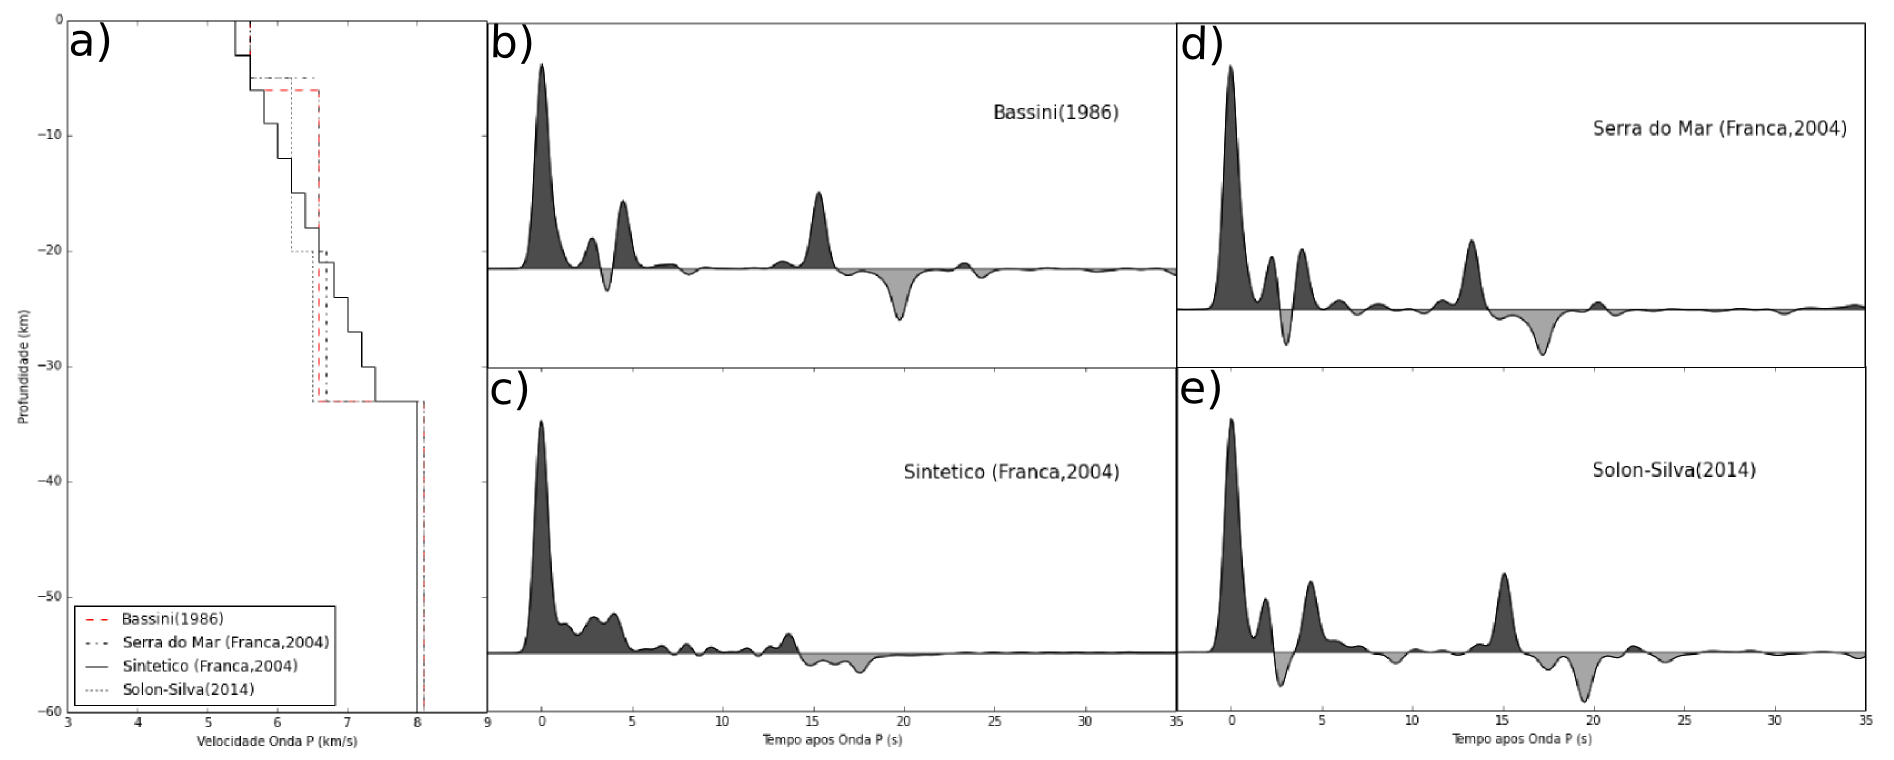
\includegraphics[scale=0.22]{Figs/modelagem_RF.png}
\caption[Funções do Receptor Sintéticas para área abrangida pelo projeto do SUBSAL]{Funções do Receptor Sintéticas para área abrangida pelo projeto do SUBSAL segundo vários tipos de modelos de velocidade da onda P. O parâmetro de largura do filtro gaussiano (a) utilizado foi 2 e o parâmetro \textit{water level} (c) foi 0.001.}
\label{modelagem}
\end{figure}

Para delimitar as principais feições estruturais da área de estudo utilizou-se de modelos de velocidade simples, 1-D, como visto na Figura \ref{modelagem}-a, apenas com camadas planas, porém tais modelos são condizentes com o contexto geológico local e são exemplos retirados da literatura sobre a região. \cite{Bassini_1986} foi o primeiro a estimar a estrutura crustual para a região da Faixa Riberia, como observado na Figura \ref{modelagem}-b). Mais tarde, \cite{sand_franca_crustal_2004} re-compilou os dados de \cite{Bassini_1986} e propôs um novo modelo de velocidade sísmica da região da Serra do Mar, como visto na Figura \ref{modelagem}-d). Recentemente \cite{flora_solon_ancient_2013} e \cite{Silva_2014} geraram resultados da estrutura crustal regional através dos métodos magnetotelúrico e gravimétrico, respectivamente. Baseando-se nesses resultados, organizou-se um modelo de velocidade sísmica para a região em estudo, como visto na Figura \ref{modelagem}-e). Uma outra opção de modelo sísmico denominado por \cite{sand_franca_crustal_2004} como modelo Sintético pode ser visto na Figura \ref{modelagem}-c). Neste modelo o autor considera que a variação das propriedades físicas da região aumenta progressivamente com a profundidade. Com esses modelos pretende-se mostrar que as estimativas da espessura crustal e razão $V_{p}/V_{s}$ são consistentes com os dados observados.

Toda a demonstração da modelagem e cálculo das Funções do Receptor sintéticas está disponibilizada por \cite{Ammon_waterlevel_1997} em \url{http://eqseis.geosc.psu.edu/~cammon/HTML/RftnDocs/rftn01.html}. Para criar os modelos de velocidade da onda $P$ utilizou-se o "\textit{icmod}", abreviação de \textit{interactive creation of model} (criação interativa de modelo). Com o modelo de velocidade criado, utilizou o programa "\textit{respknt}" para calcular numericamente a resposta da estrutura para um onda P incidente. Este programa é baseado na matriz de reflexão de \cite{kennett_seismic_1983}, que computa a resposta sísmica de um meio cilíndrico simétrico. Após o cálculo numérico da resposta da estrutura, o programa "\textit{pwaveqn}" calcula as Funções do Receptor no domínio da frequência para os modelos pré-estabelecidos. O programa "\textit{pwaveqn}" exige como dados de entrada a determinação do parâmetro \textit{water level} e a banda de frequência a ser utilizada. Os parâmetros utilizados para o cálculo das Funções do Receptor estão na Figura \ref{modelagem}.

As Funções do Receptor sintéticas apresentadas na Figura \ref{modelagem} mostram uma reflexão característica em torno de 5 segundos onde a onda $P$ se converte em $S$ (primeira reflexão de Moho), como mostra \cite{langston_structure_1979}. Antes dessa reflexão é notável um pulso senoidal em torno de 2.5 segundos nas Figuras \ref{modelagem}-b), \ref{modelagem}-d) e \ref{modelagem}-e). Este pulso está relacionado com a camada superficial de baixa velocidade. Tal camada possui espessura aproximada de 5 quilômetros, análoga a uma bacia sedimentar. No contexto local pode ser representada como a Bacia de Taubaté na região da Faixa Ribeira. As outras reverberações de Moho são bem características, essas múltiplas $PpPs$ e $PpSs+PsPs$ são bem demarcadas em $\sim 13$ e $\sim 19$ segundos neste modelo de velocidade.

Os resultados gerados pelos modelos de velocidade mostram como as Funções do Receptor se comportam a algumas variações de velocidade. Nota-se que quando as variações de velocidades são grandes pode-se visualizar melhor a conversão da onda $P$ em $S$ e suas múltiplas, como visto nas Figuras \ref{modelagem}-b), \ref{modelagem}-d) e \ref{modelagem}-e). Porém quando há uma pequena variação da velocidade com a profundidade, como exemplo o modelo Sintético de \cite{sand_franca_crustal_2004}, a identificação das reflexões na Função do Receptor é bem complicada, como pode ser visto na Figura \ref{modelagem}-c).

\subsection{Modelos de velocidade perfilados para camadas inclinadas}

\begin{figure}[!ht]
\centering
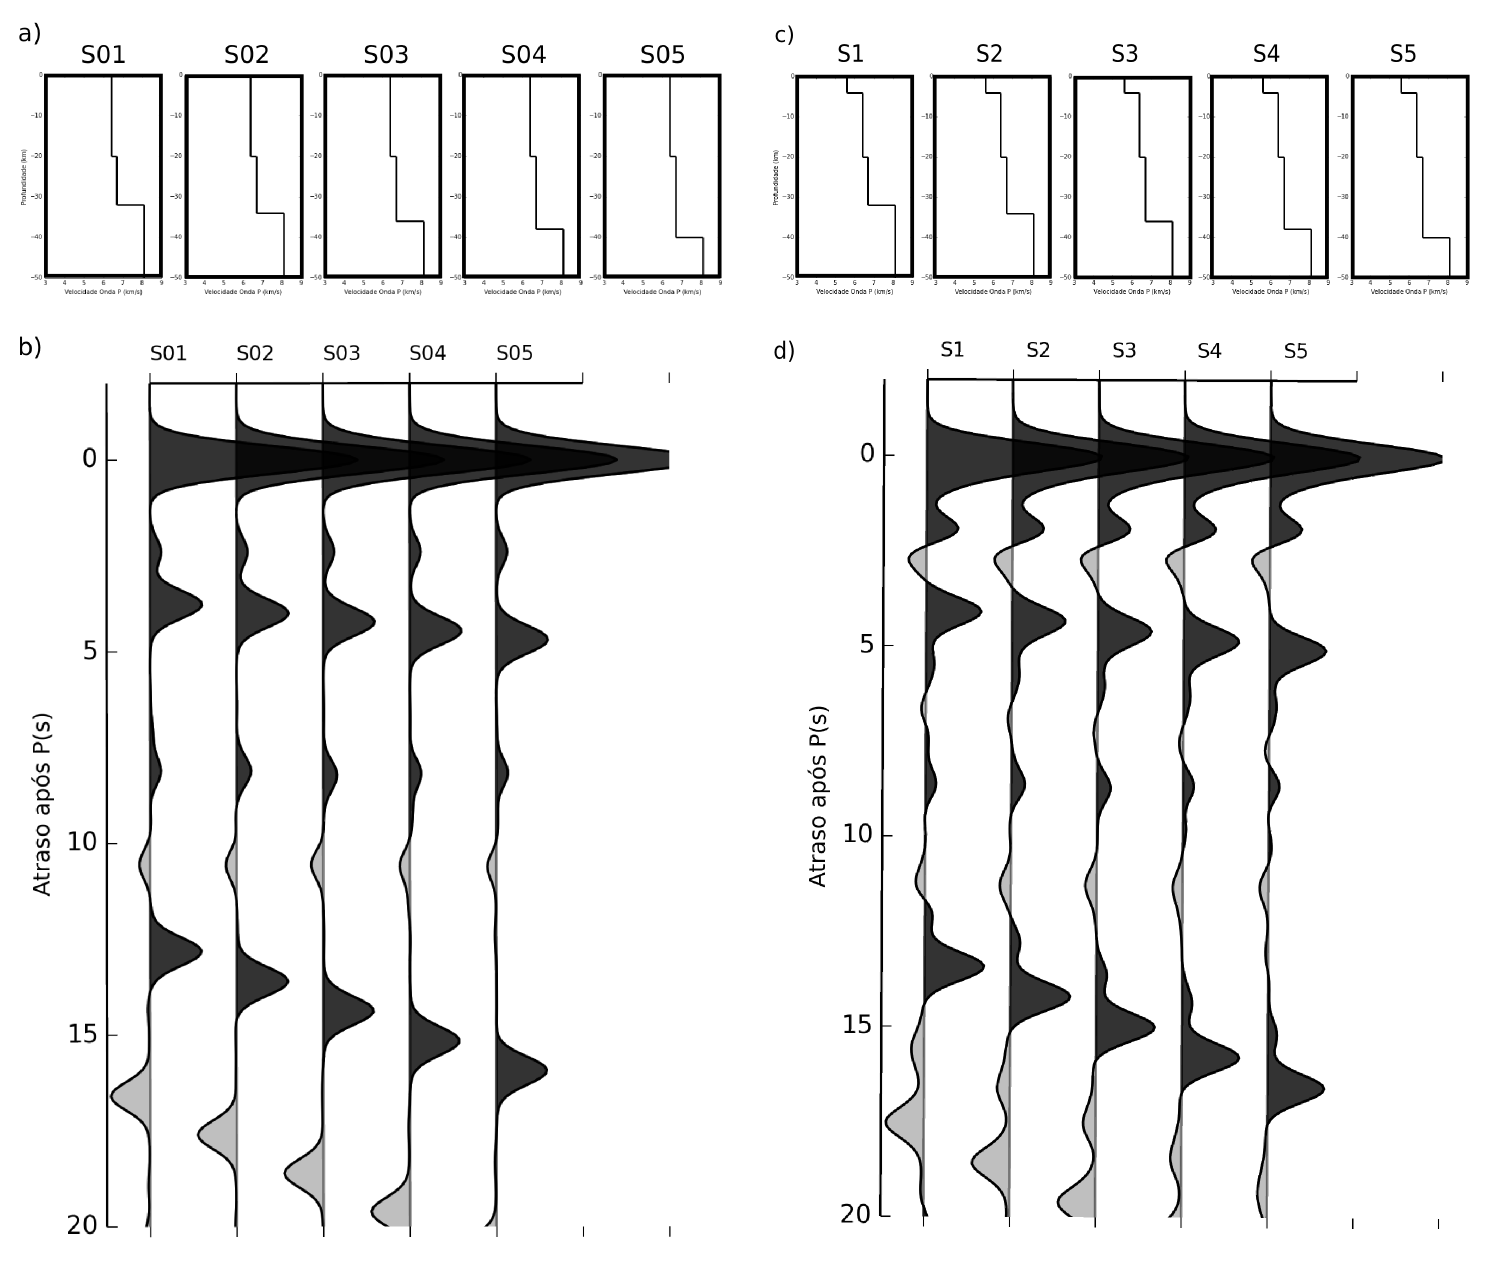
\includegraphics[scale=0.25]{Figs/perfil_RF_sintetico.png}
\caption[Perfil com Funções do Receptor Sintéticas para área abrangida pelo projeto do SUBSAL]{Perfil com Funções do Receptor Sintéticas para área abrangida pelo projeto do SUBSAL segundo modelos de velocidade Solon-Silva(2014), como mostrado na Figura \ref{modelagem}.}
\label{perfil_modelagem}
\end{figure}

Para entender melhor como as Funções do Receptor são influenciadas por uma configuração estrutural mais complexa, modelos de velocidade sintéticos foram perfilados para gerar dados semelhantes aos da Rede SUBSAL. Esses modelos apresentam profundidades diferentes de Moho para cada estação, além de um descontinuidade intermediária. Isto é feito para entender a resposta da Função do Receptor para tais profundidades, como mostrado na Figura \ref{perfil_modelagem}-a). O modelo apresentado na Figura \ref{perfil_modelagem}-c) apresenta uma camada superficial com baixa velocidade  e na Figura \ref{perfil_modelagem}-e) introduziu-se uma inversão de velocidade no perfil criado para analisar a resposta das Funções do Receptor neste tipo estruturação crustal.

Na Figura \ref{perfil_modelagem} observa-se três grupos de perfis de modelos com velocidades diferentes. Tais modelos foram confeccionados de acordo com o modelos geológicos locais e com os perfis de velocidades citados anteriormente. A Figura \ref{perfil_modelagem}-a) mostra os perfis de velocidade baseados nas inversões de \cite{flora_solon_ancient_2013} e de \cite{Silva_2014} com uma descontinuidade constante bem marcada no meio da crosta, por volta de $20 \sim km$. A resposta dessa descontinuidade média da crosta é apresentada na Figura \ref{perfil_modelagem}-b). Onde também é mostrado uma descontinuidade de Moho variando de profundidade em cada estação, bem marcada pela distância entre a primeira reflexão e a segunda grande reflexão, conversão da onda P em S.

Nos modelos de velocidade apresentados na Figura \ref{perfil_modelagem}-c) é adicionado uma camada com baixa velocidade na parte superior do perfil, de profundidade $5 km$, analogamente à bacias sedimentares terciárias presentes na área, como a Bacia de Taubaté. A resposta a essa camada de baixa velocidade é mostrada na Figura \ref{perfil_modelagem}-c) como um pulso senoidal por volta de 2,5 segundos.

Na Figura \ref{perfil_modelagem}-e) adicionou-se ao modelo de velocidade uma velocidade alta na parte superior da crosta com inclinação contrária a descontinuidade caracterizada com Moho. Nota-se na Figura \ref{perfil_modelagem}-f) que há uma sobreposição de sinais referentes a essas essa descontinuidades. Logo quanto maior a complexidade da área há uma dificuldade na interpretação dos resultados da Funções do Receptor.

\section{Resultados}

Pesquisas envolvendo a propagação de ondas sísmicas no interior da Terra auxiliam na determinação da estrutura da mesma. Essas análises permitem recuperar, dependendo da resolução, a geometria das descontinuidades no interiores, ligadas à velocidade de propagação das ondas de corpo.  

O método da Função do Receptor, desenvolvido por \cite{Langston_1977}, gera informações sobre a estrutura debaixo da estação sismográfica. A confiança nos resultados gerados pelo método varia em função da quantidade e qualidade das Funções do Receptor. Por isso é importante que a estação esteja funcionando corretamente e tenha uma grande quantidade de dados disponíveis.

O foco principal deste trabalho foram as fases da Função do Receptor relacionadas a descontinuidade de Moho, interface Crosta-Manto, e reflexões internas da crosta terrestre. Os resultados obtidos pelas estações temporárias foram comparados com a estação SLP01, estação permanente próxima a região de estudo. Assim aumentando a confiabilidade nos dados gerados pela rede de estações temporárias.

\begin{figure}[!ht]
\centering
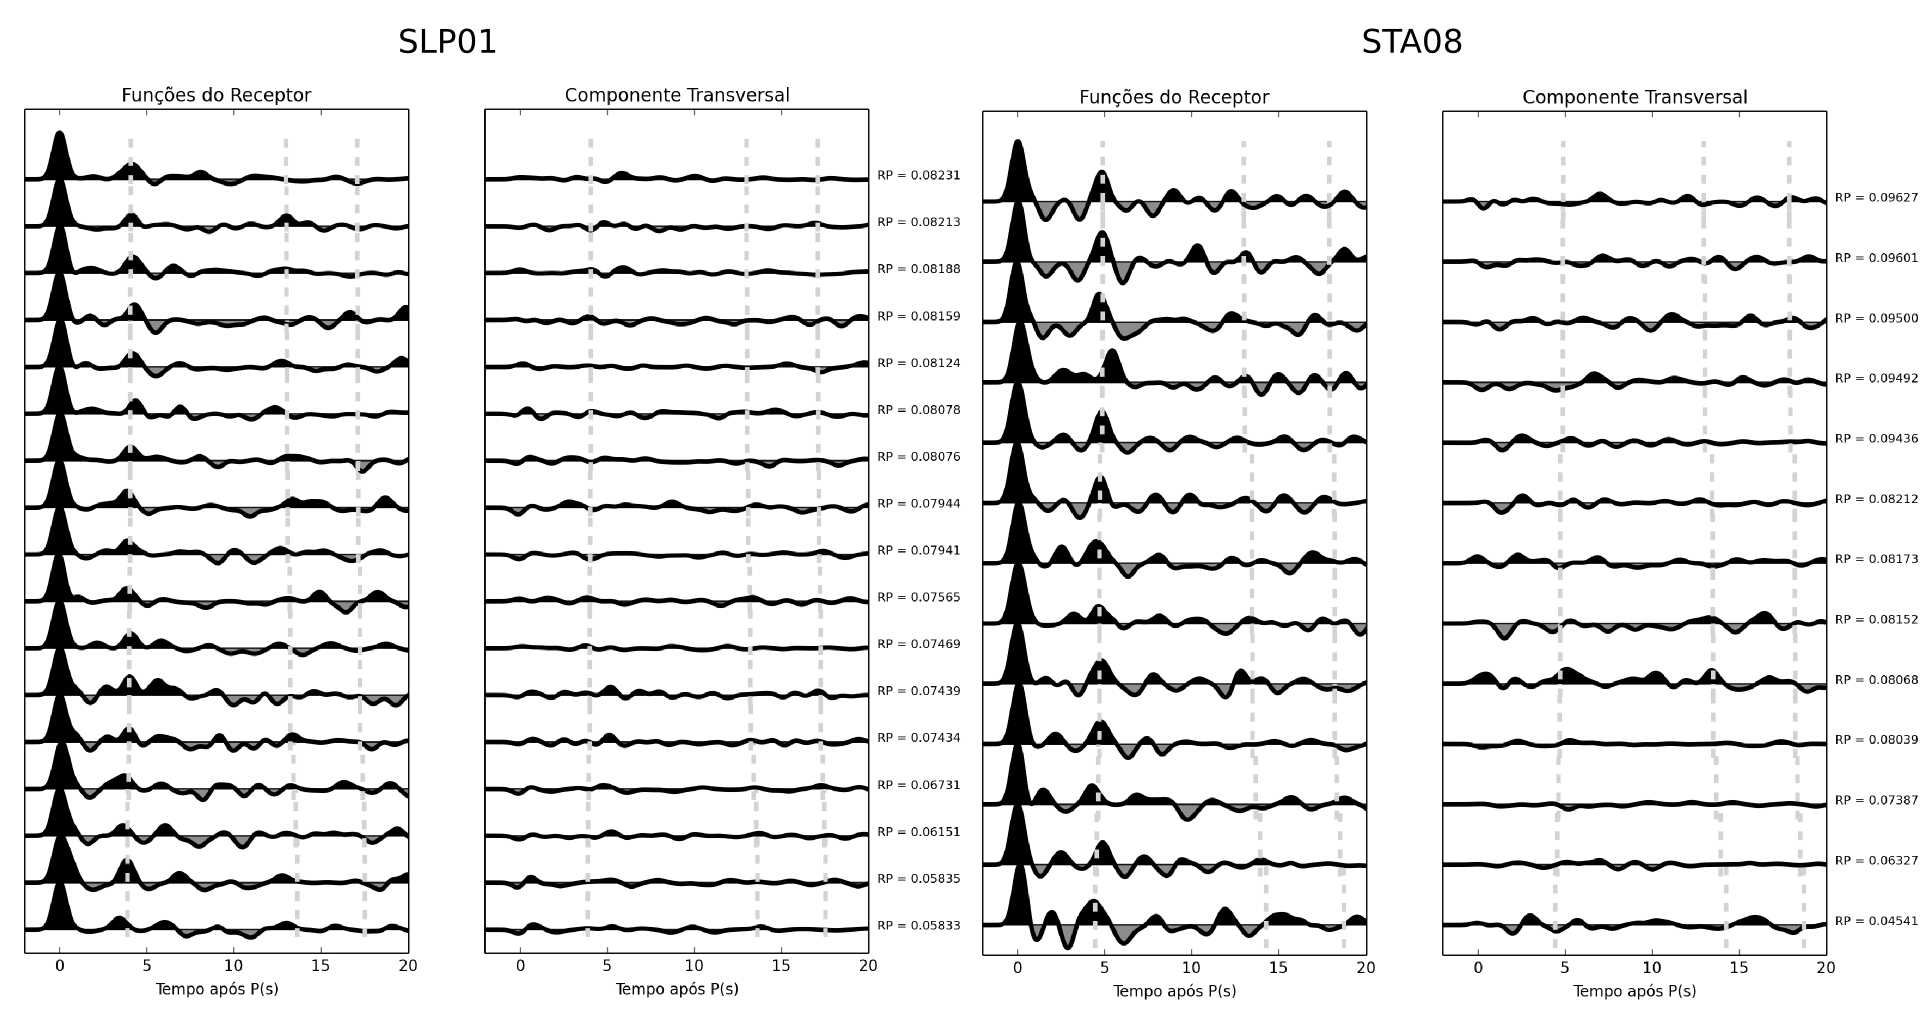
\includegraphics[scale=0.16]{Figs/RF_SLP01_STA08.png}
\caption[Exemplos de Funções do Receptor e da Componente Transversal para as estações SLP01 (permanete) e STA08 (temporária)]{Exemplos de Funções do Receptor e da Componente Transversal para as estações SLP01(permanete) e STA08(temporária) distribuídas em função do parâmetro do Raio. O primeiro pico significa a chegada da onda $P$ direta. Já o segundo a conversão da onda $P$ em $S$ em Moho. As outras múltiplas geradas em Moho não são observáveis. A linha pontilhada simboliza os tempos de chegada teóricos calculados segundo o modelo IASPEI91 de \cite{kennet_iaspei_1991}. O parâmetro de largura do filtro gaussiano (a) utilizado foi 2 para sismos distantes ($>$20º) e de 15 para sismos próximos ($<$20º). }
\label{RF_SLP01_STA08}
\end{figure}

A Figura \ref{RF_SLP01_STA08} mostra as Funções do Receptor obtidas a partir de vários eventos para a estação permanente SLP01 e para a estação temporária STA08, estas organizadas de acordo com o parâmetro do raio. Estes sinais foram normalizados pela amplitude do primeiro pico, que é a chegada da onda P direta, já o segundo, por volta de 5 segundos, é a onda P convertida em onda S na descontinuidade de Moho. As linhas verticais pontilhadas demarcam os tempos teóricos de chegada calculados pelo modelo IASPEI91 de \cite{kennet_iaspei_1991} para cada múltipla. As multiplas $PpPs$ e $PpSs+PsPs$ tem uma amplitude menor que a onda P convertida em S ($Ps$) devido a grande distância entre o ponto incidente e a estação, então estas reverberações são mais afetadas por variações laterias, espallhamento e atenuação inelástica. Os sismogramas não apresentam clareza quanto a essas reverberações. A múltipla $PpPs$ não é observada facilmente e a múltipla $PpSs+PsPs$ está mascarada pelo ruído em todos os registros das estações temporárias.

Com as Funções do Receptor calculadas, utilizou-se a método desenvolvido por \cite{Zhu_Kanamori_2000} para calcular a profundidade de Moho e a razão $v_{p}/v_{s}$ nas estações sismográficas. Os resultados gerados estão descritos na Tabela \ref{tabelaMoho} (Anexo 2). Para uma melhor visualização dos resultados gerados interpolou-se as profundidades de Moho. Para melhorar a distribuição espacial das profundidades adicionou-se algumas estações sismográfica utilizados por \cite{Assumpcao_Brazil_2013}, estações localizadas na Tabela \ref{tabelaDATAcorr}. O mapa da interpolação das medidas das espessuras de Moho pode ser visto na Figura \ref{Interpolacao}. Nota-se na Figura \ref{Interpolacao} que a descontinuidade de Moho estimada é maior no interior do continente do que na região costeira, corroborando com os dados de \cite{sand_franca_crustal_2004}, \cite{Assumpcao_America_2013}, \cite{Assumpcao_Brazil_2013} e \cite{van_der_meijde_gravity_2013}. As estações que bordeiam o Cráton do São Francisco e a Bacia do Paraná tem uma espessura média de Moho de 40 km. Já as outras estações tendem a uma espessura de Moho crescente quando mais próximas da Faixa Brasília, Cráton do São Francisco e da Bacia do Paraná.

\begin{figure}[!ht]
\centering
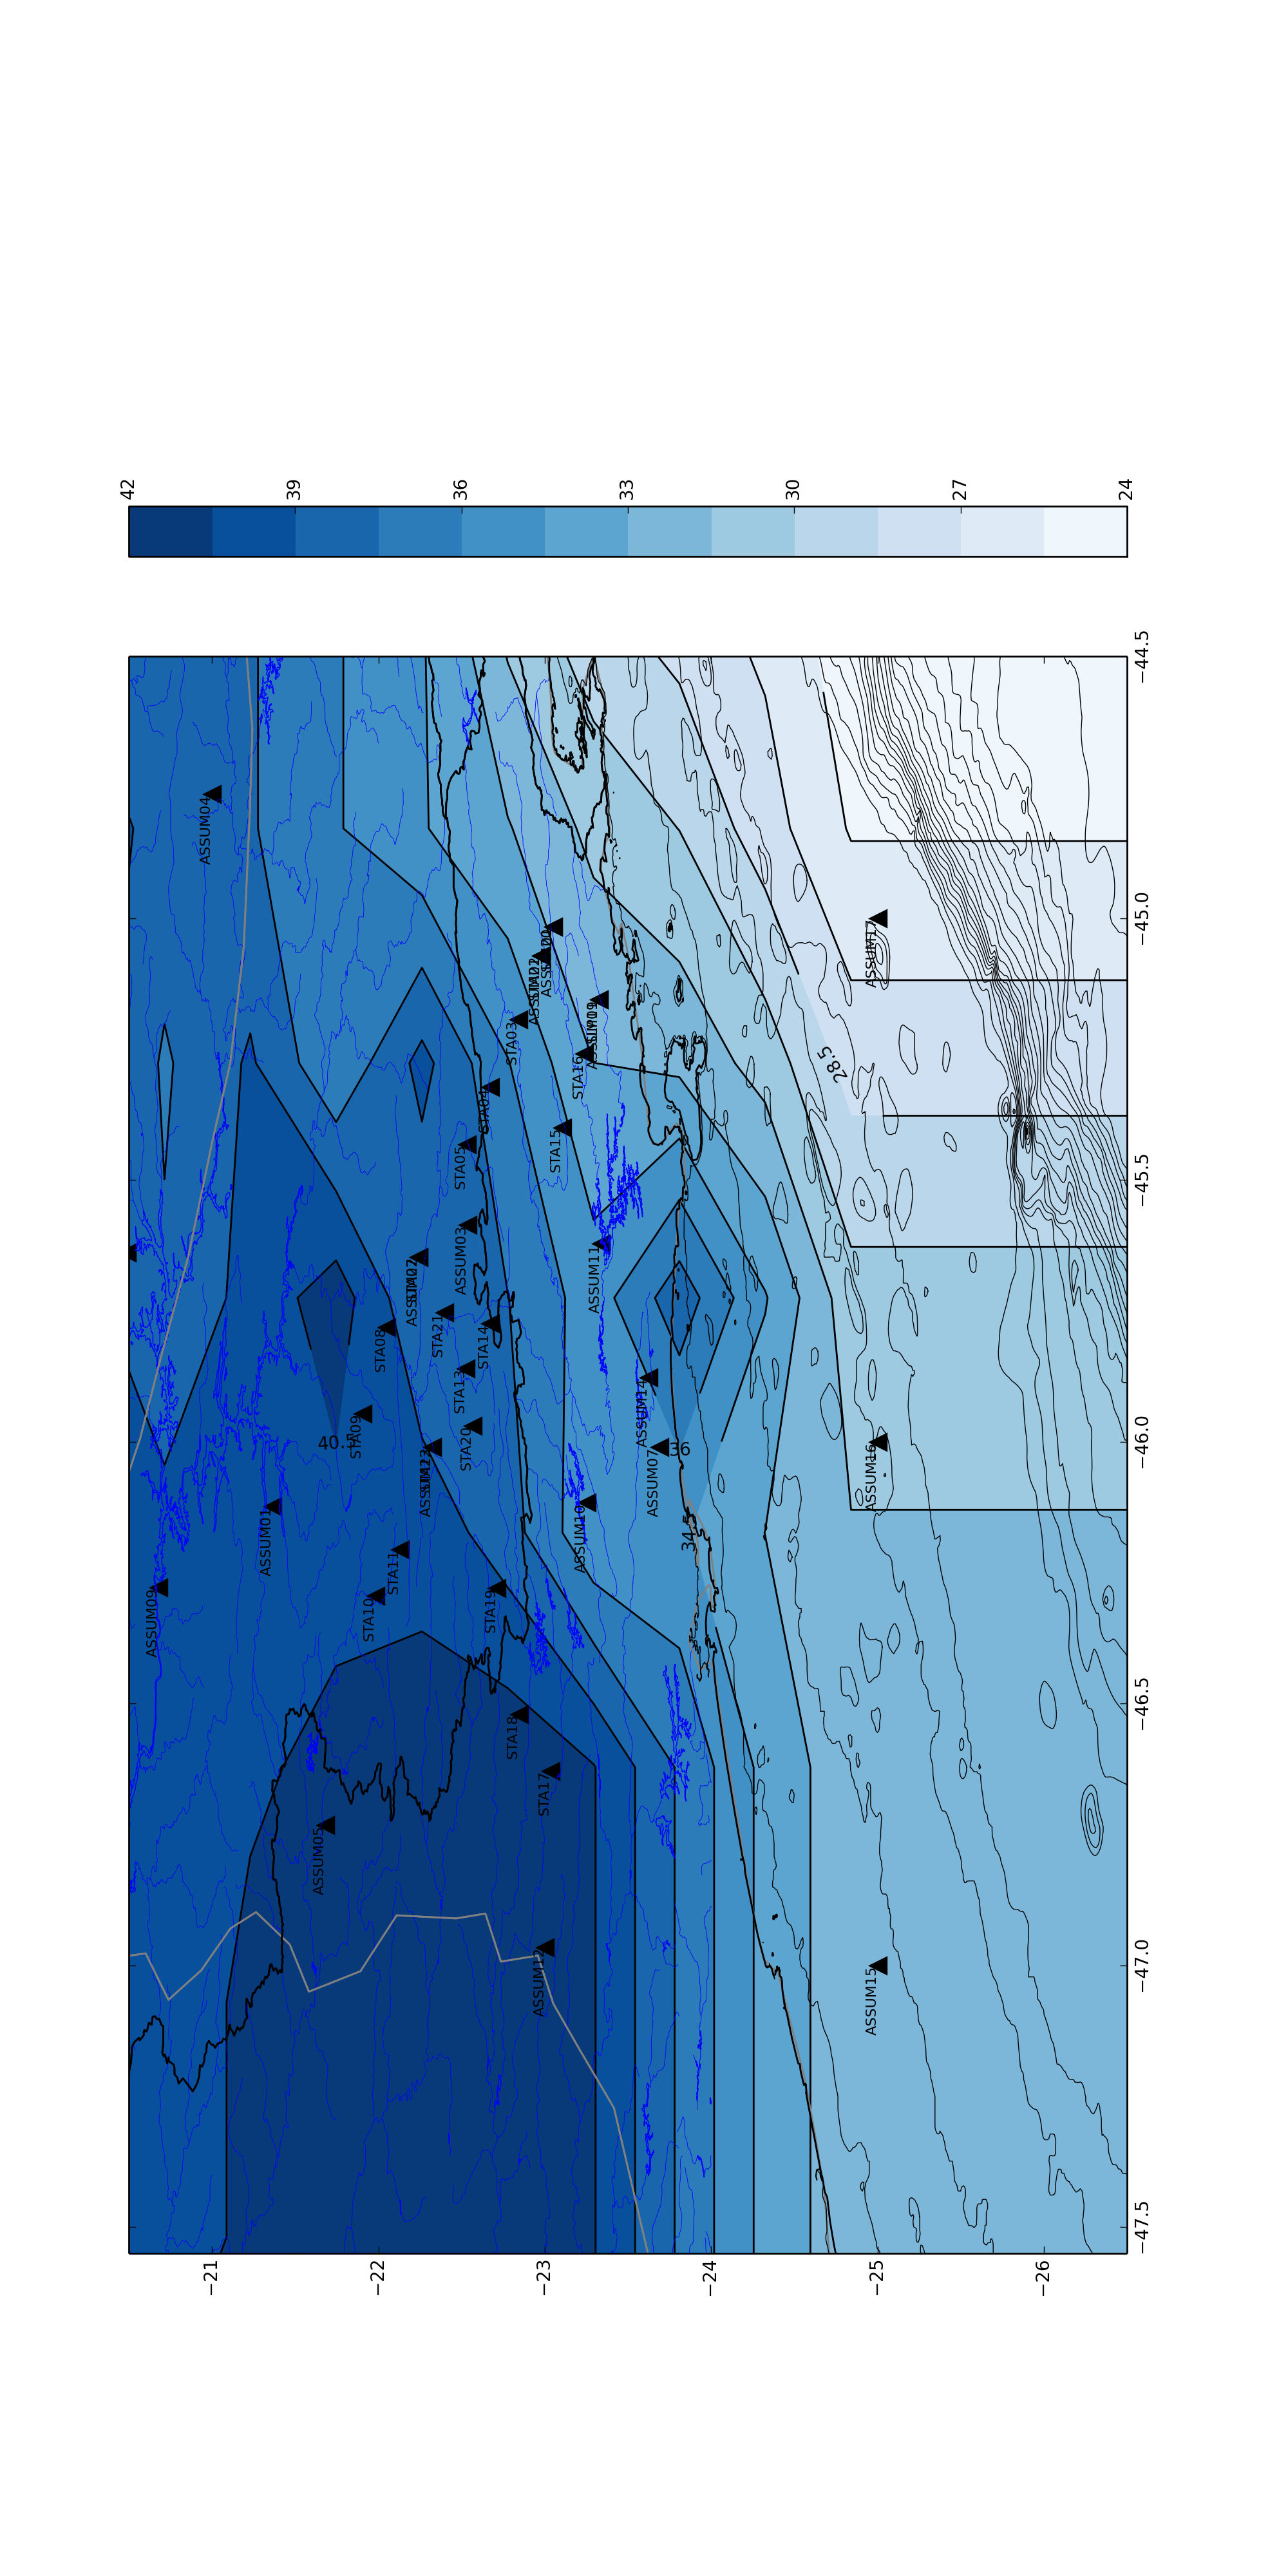
\includegraphics[scale=1]{Figs/Interpolacao_Linear.png}
\caption[Mapa da espessura crustal da região em estudo.]{Mapa da espessura crustal da região em estudo, os valores da espessura de Moho está localizado na Tabela \ref{tabelaMoho} (Anexo 2). Os círculos representam as estações sismográficas e as cores represetam a espessura de Moho em cada estação. O tamanho do círculo em cada estação representa a influência do erro, quanto maior o círculo menor o erro da profundidade de Moho para a estação. BP-Bacia Paraná, CSF-Cráton do São Francisco, FB-Faixa Brasília, TO-Terreno Oriental  e FR-Faixa Ribeira.}
\label{Interpolacao}
\end{figure}

O mapa gerado pela interpolação das razões $V_{p}/V_{s}$ para cada estação pode ser visto na Figura \ref{Interpolacao_vpvs}. As razões $V_{p}/V_{s}$ estão na  \ref{tabelaMoho} (Anexo 2). Pode ser visto na  Figura \ref{Interpolacao_vpvs} que a média da razão $V_{p}/V_{s}$ para a região em estudo é por volta de 1.73 a 1.75. Não há um padrão bem estabelecido para a razão $V_{p}/V_{s}$ e as estruturas geológicas da região, porém o que é pode ser distinguido é que próximo a costa da divisa entre o Rio de Janeiro e São Paulo a razão $V_{p}/V_{s}$ é maior que nas outras regiões.

\begin{figure}[!ht]
\centering
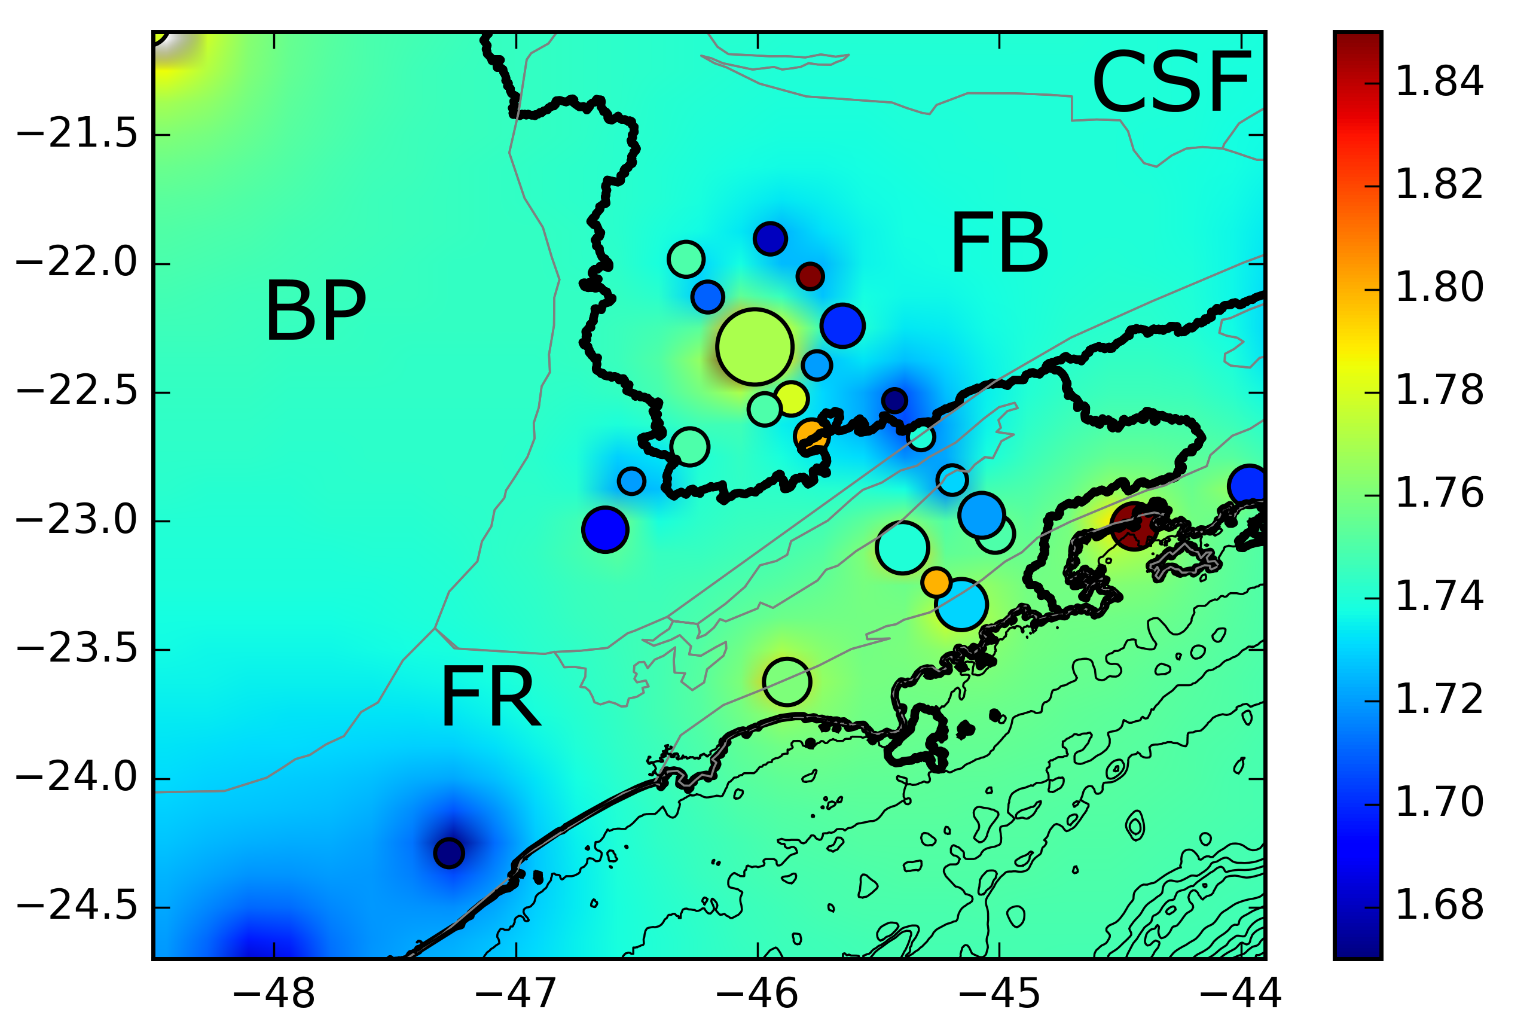
\includegraphics[scale=1]{Figs/Interpolacao_Linear_vpvs.png}
\caption[Interpolação da razão $V_{p}/V_{s}$ para cada estação.]{Interpolação da razão $V_{p}/V_{s}$ para cada estação. Os círculos representam as estações sismográficas e as cores represetam a razão $V_{p}/V_{s}$ em cada estação. O tamanho do círculo em cada estação representa a influência do erro, quanto maior o círculo menor o erro da razão $V_{p}/V_{s}$ para a estação. BP-Bacia Paraná, CSF-Cráton do São Francisco, FB-Faixa Brasília, TO-Terreno Oriental  e FR-Faixa Ribeira.}
\label{Interpolacao_vpvs}
\end{figure}

As Funções do Receptor para cada estação foram empilhadas linearmente para gerar estes perfis, de acordo com o arranjo das estações sismográficas. 
Os perfis mostrados nas Figuras \ref{RF_perfil1}, \ref{RF_perfil2} e \ref{RF_perfil3} reforçam  os resultados mostrados na Figura \ref{Interpolacao}. Observando estes perfis é evidente que a proximidade com a costa  faz com que as reflexões tendam a ser mais rápidas devido a menor espessura de Moho, logo ratificando o afinamento crustal na direçãodo oceano. No perfil paralelo a costa, Figura \ref{RF_perfil3}, nota-se uma tendência de afinamento crustal em direção a Bacia do Paraná, porém uma variação lateral pequena. 

Identificam-se sinais precursores ao sinal de Moho por volta de 2 a 4 segundos, estes variam ao longo de todos os perfis, como pode ser visto nas Figuras \ref{RF_perfil1}, \ref{RF_perfil2} e \ref{RF_perfil3}. Estes sinais apresentam-se na forma de senoídes, e de acordo com as modelagens apresentadas nas Figuras \ref{modelagem} e \ref{perfil_modelagem} podem ser relacionados com uma interface superficial de baixa velocidade. É visível a mudança no comportamento desses sinais de acordo com o grupo de backazimute, corroborando sobre a heterogeneidade geológica da região. \cite{vinnik_depth_2007} mostra que na presença de anisotropia azimutal ou heterogeneidade lateral, as ondas convertidas e refletidas são registradas em todas todas as três componentes e suas amplitudes dependem do azimute. Pode ser observado na Figura \ref{RF_SLP01_STA08} altas amplitudes na componente tangencial das Funções do Receptor de ambas estações. Segundo \cite{vinnik_depth_2007}, se as fases convertidas e reverberadas na componente radial das Funções do Receptor possuem amplitudes maiores que as fases da componente tangencial, a aproximação 1-D para a estrutura abaixo da estação é considerada válida.

\begin{figure}[!ht]
\centering
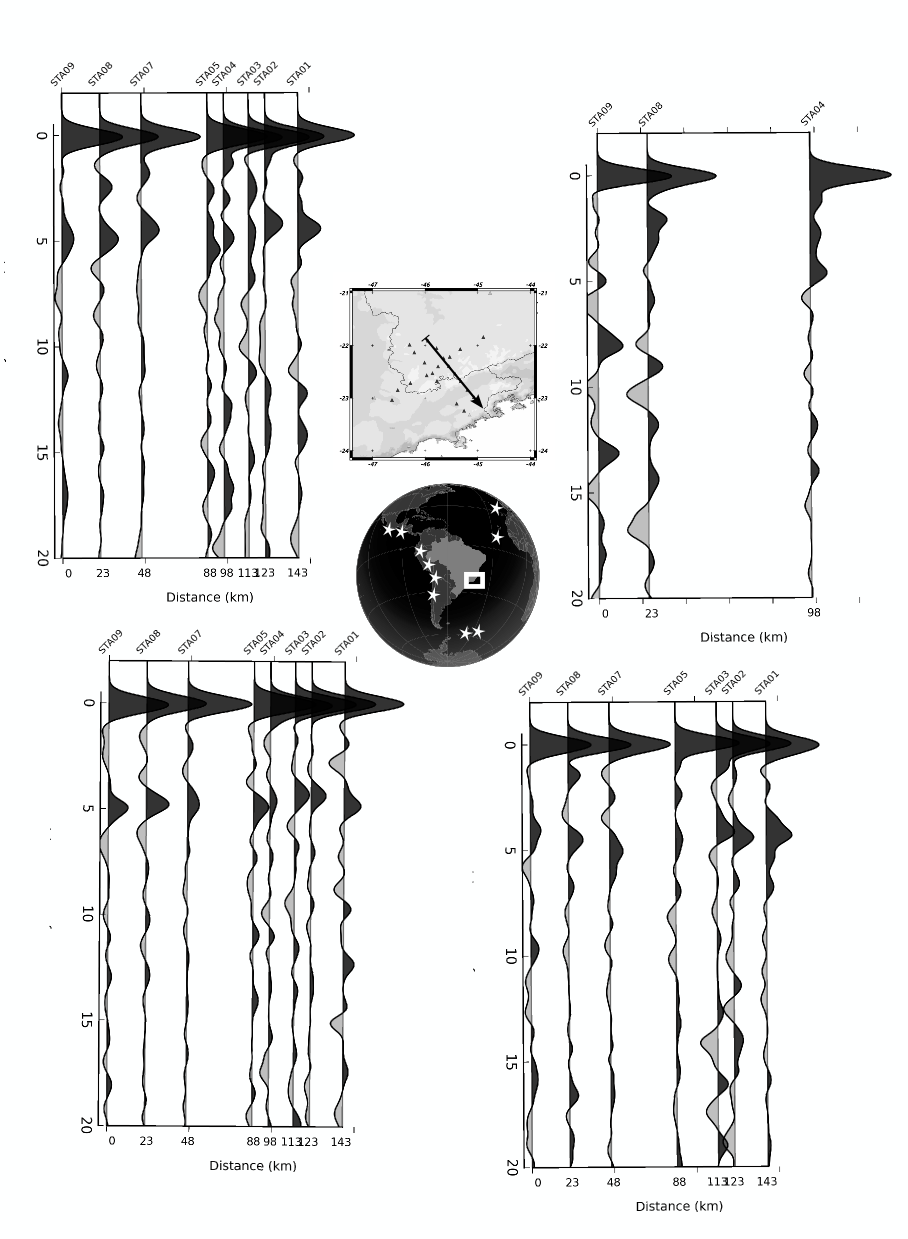
\includegraphics[scale=0.5]{Figs/RF_azimute_perfil1.png}
\caption{Seção com as Funções do Receptor empilhadas linearmente segundo o perfil 1 (STA09-STA01). Cada traço foi empilhado linearmente de acordo com seu grupo de backazimute: NE,SE,SW e NW.}
\label{RF_perfil1}
\end{figure}

\begin{figure}[!ht]
\centering
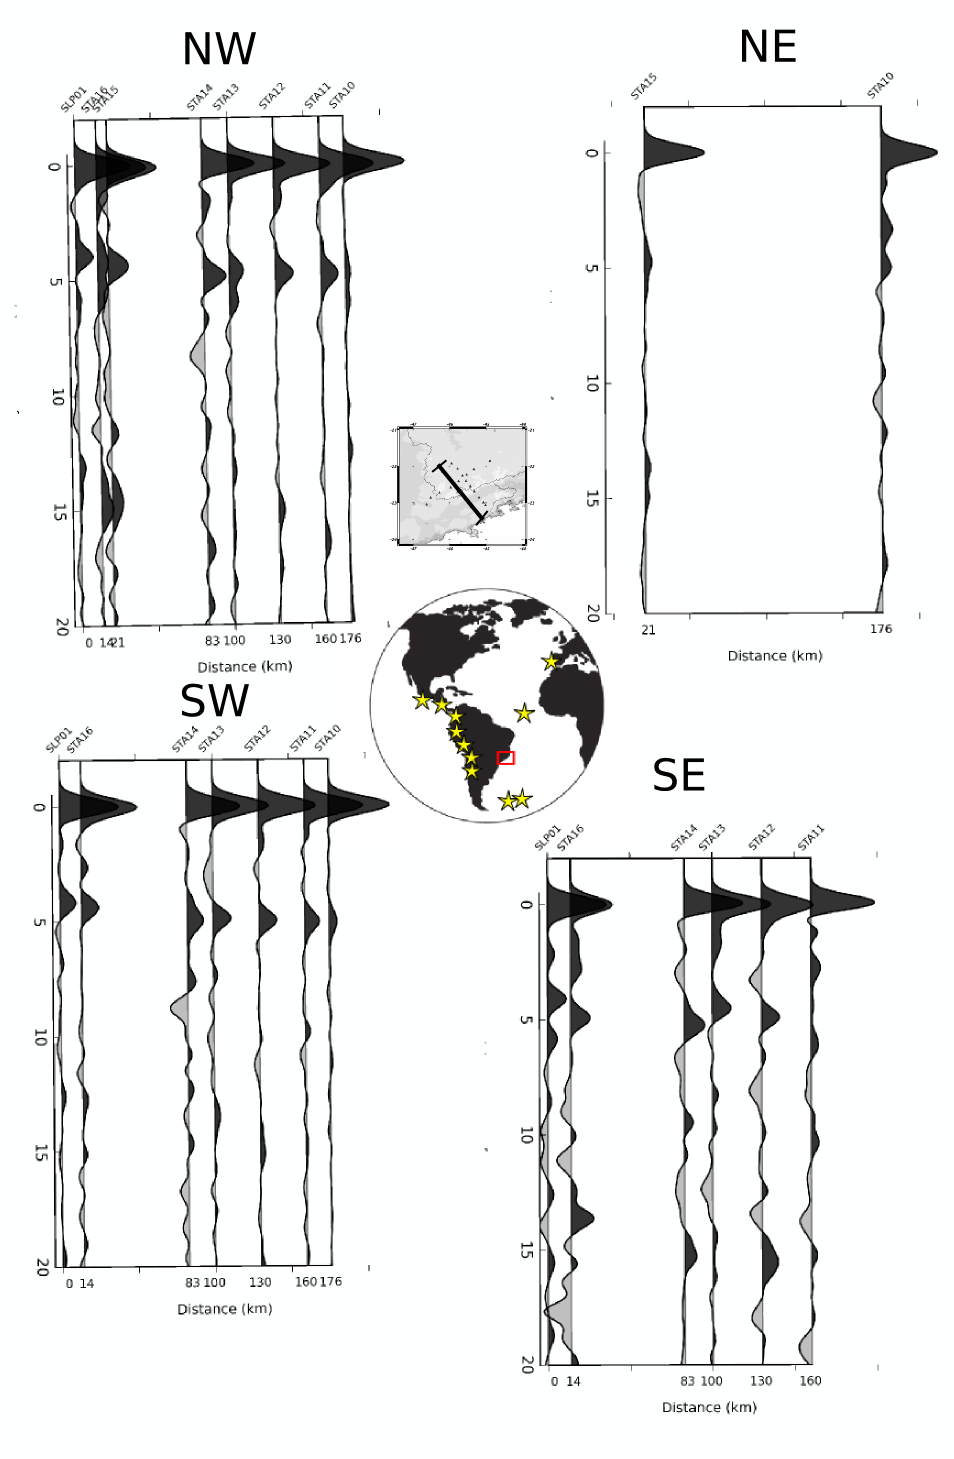
\includegraphics[scale=0.5]{Figs/RF_azimute_perfil2.png}
\caption{Seção com as Funções do Receptor empilhadas linearmente segundo o perfil 2 (STA10-SLP01). Cada traço foi empilhado linearmente de acordo com seu grupo de backazimute: NE, SE, SW e NW.}
\label{RF_perfil2}
\end{figure}

\begin{figure}[!ht]
\centering
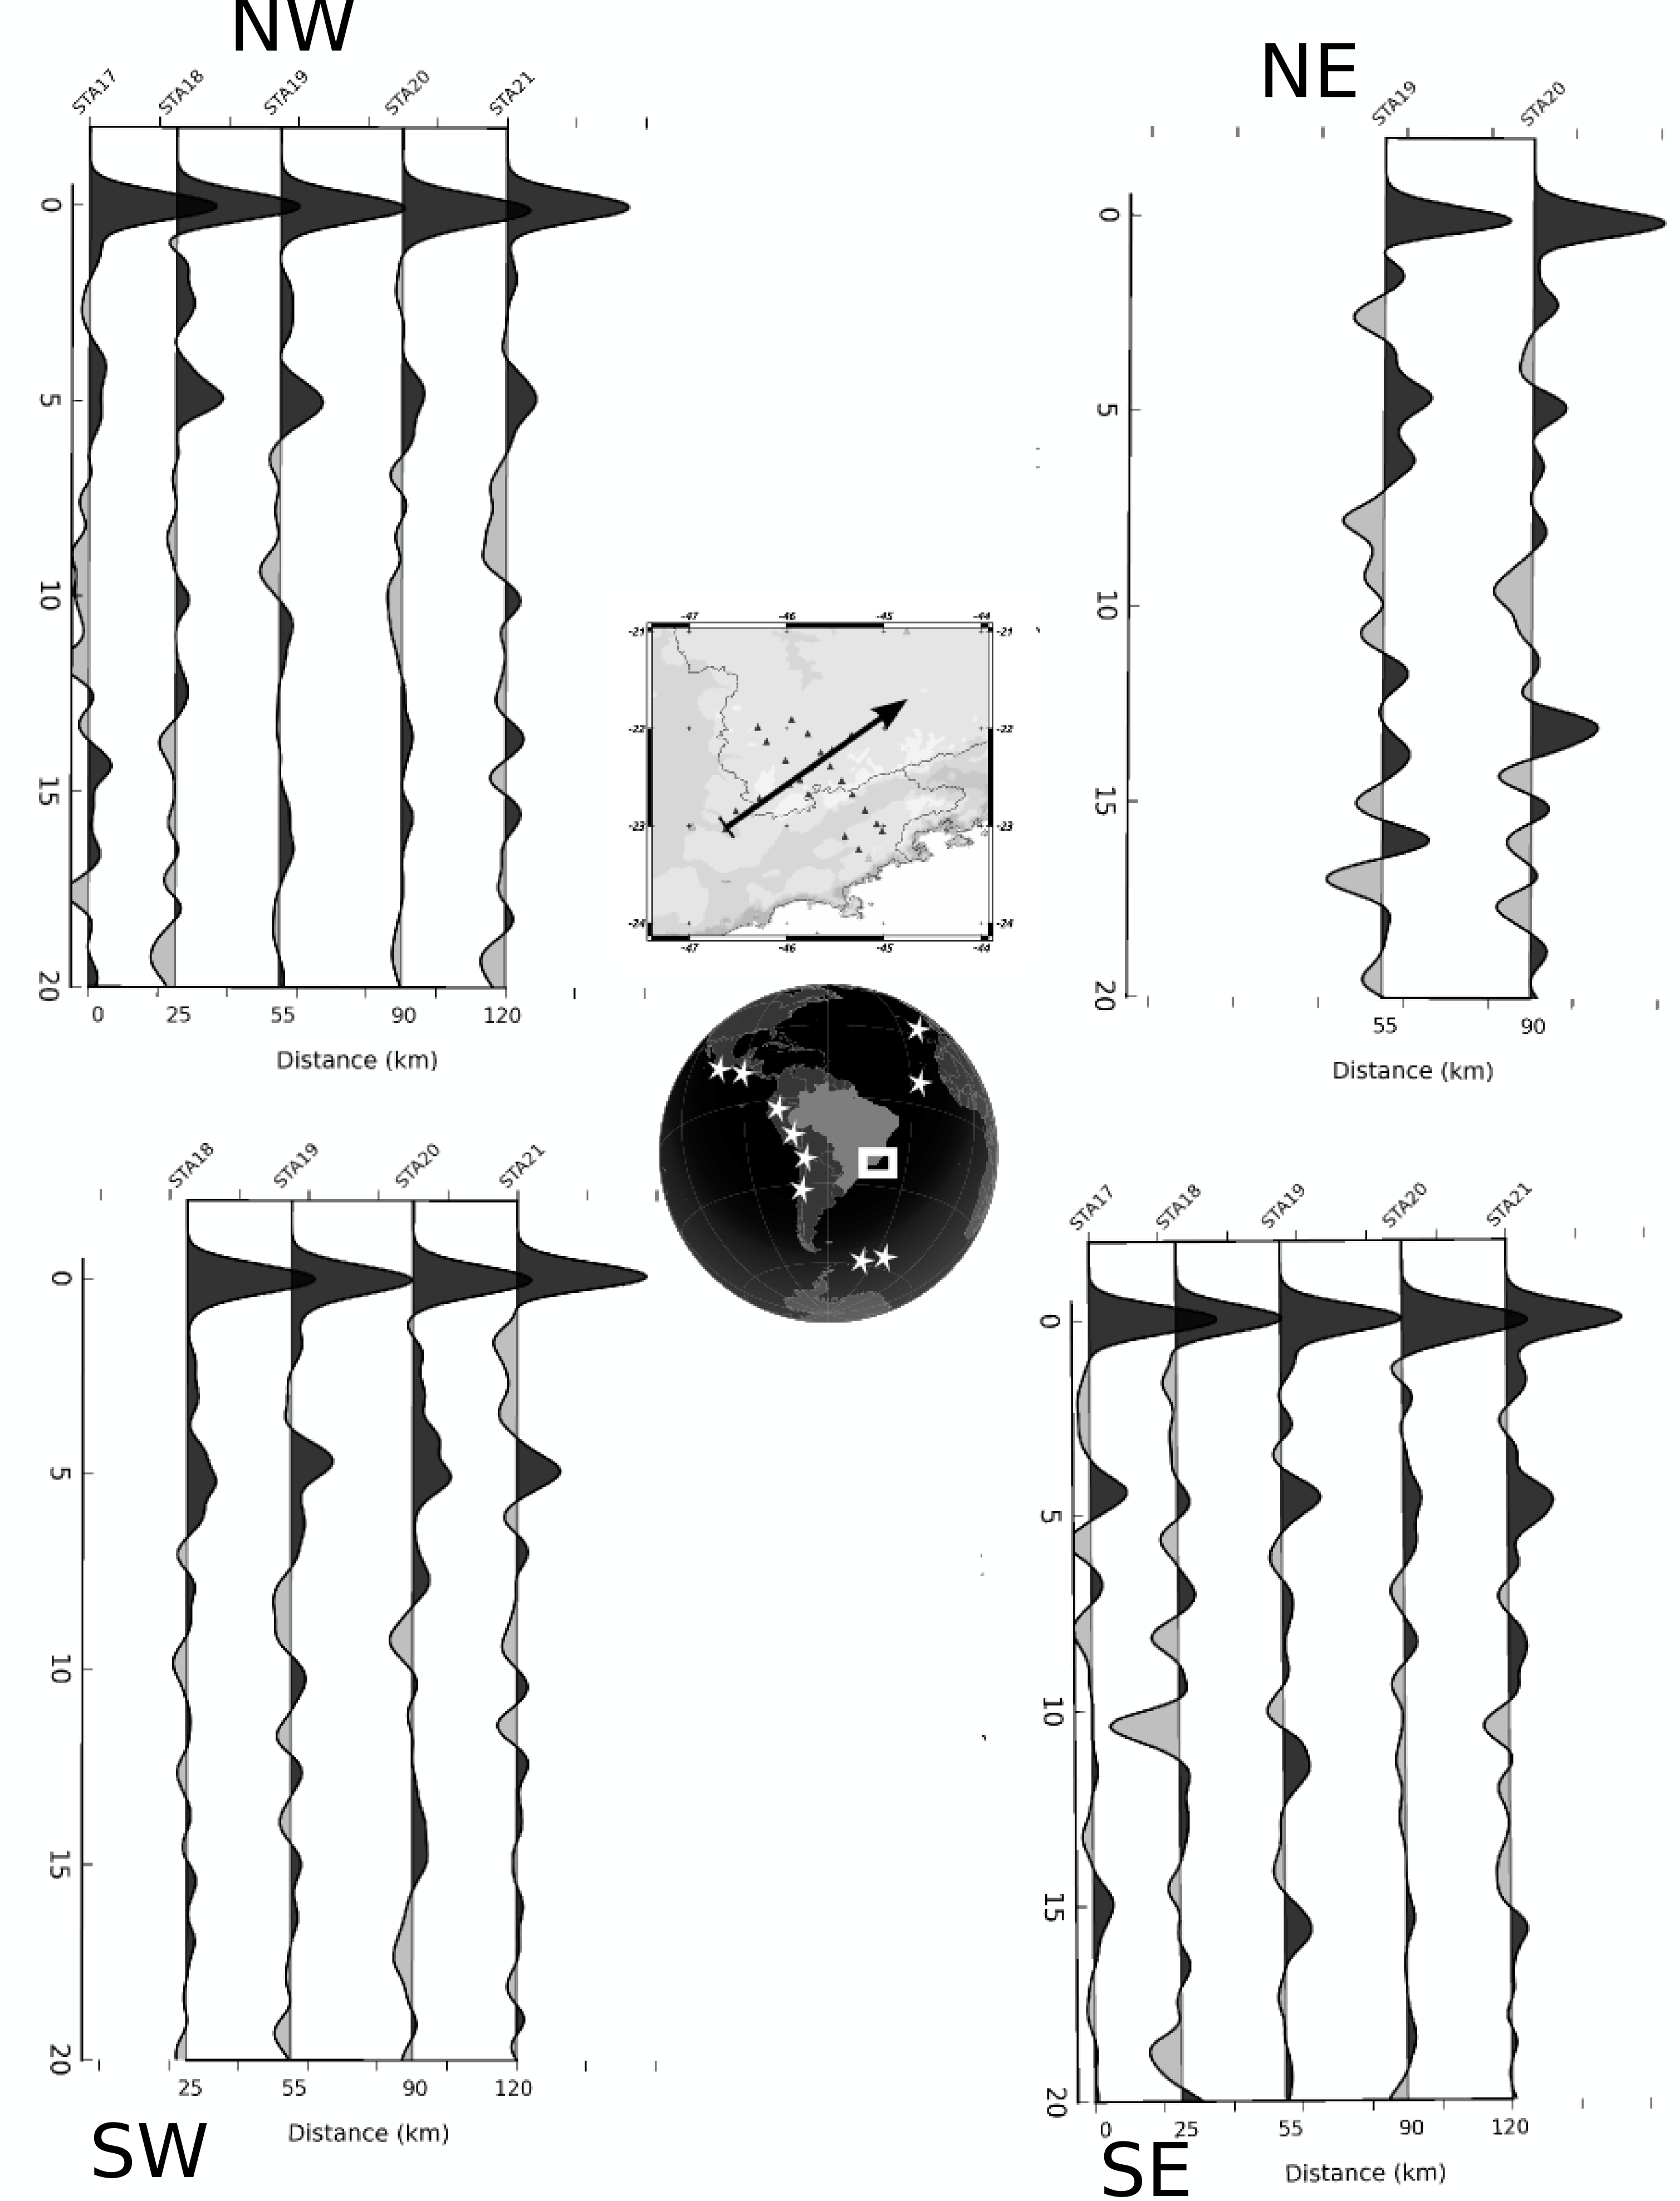
\includegraphics[scale=0.5]{Figs/RF_azimute_perfil3.png}
\caption{Seção com as Funções do Receptor empilhadas linearmente segundo o perfil 3 (STA17-STA21). Cada traço foi empilhado linearmente de acordo com seu grupo de backazimute: NE, SE, SW e NW.}
\label{RF_perfil3}
\end{figure}

Analisando os traços das Figuras \ref{RF_perfil1}, \ref{RF_perfil2} e \ref{RF_perfil3} nota-se uma diferença considerável na qualidade das Funções do Receptor para cada grupo de azimute. Além da quantidade de eventos oriundos da parte oriental (NE e SE) ser menor que a ocidental, que gera Funções do Receptor de baixa qualidade, observa-se nos tracos do grupo NE um sinal semelhante com o modelo Sintético mostrado por \cite{sand_franca_crustal_2004}, Figura \ref{modelagem}-c), em que há inúmeros pontos causadores de espalhamento. Isso gera um sinal bastante sinuoso sem marcações claras das reflexões e reverberações de Moho.

Visando diminuir o ruído e melhorar a interpretação visual do resultadso das Funções do Recepetor incrementou-se o método desenvolvido por \cite{schimmel_noise_1997} através do janelamento. O resultado pode ser visto na Figura \ref{LS_PWSW}. É notável supressão de sinal após 15 segundos e também que em nenhuma das estações há reverberações de Moho visíveis. Uma observação importante é a presença de picos positivos antes de 5 segundos após a utilização da PWSW, e também existe um conjunto de picos negativos entre 5 e 10 segundos que possuem um padrão de reflexão contrário a Moho. Estas reflexões podem estar relacionadas a uma descontinuidade interna á crosta.

\begin{figure}[!ht]
\centering
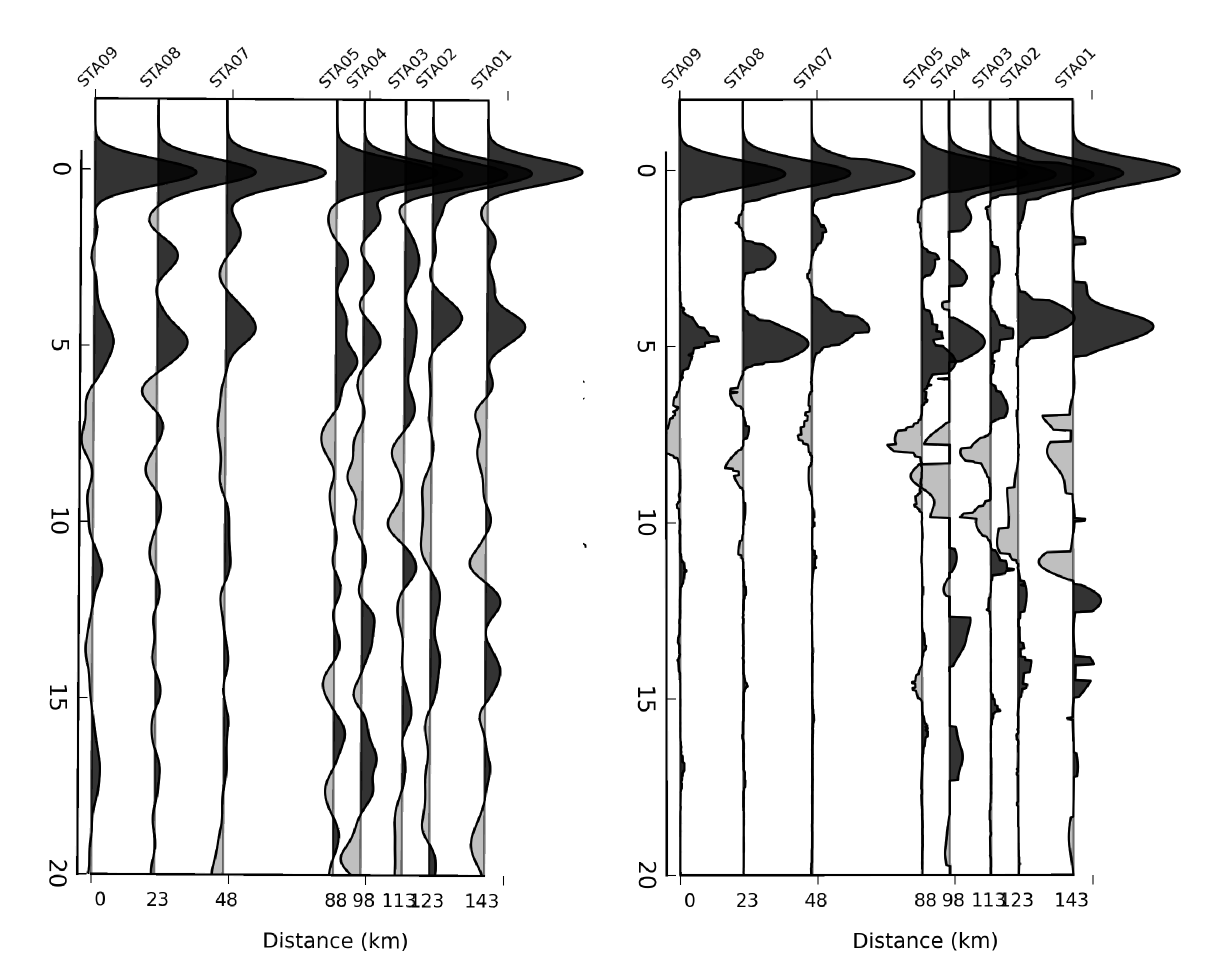
\includegraphics[scale=0.25]{Figs/comp_ls_pwsw.png}
\caption{Seções do perfil 1 do grupo NW comparando entre os métodos de empilhamento linear (LS) e empilhamento ponderado na fase com janelamento (PWSW)}
\label{LS_PWSW}
\end{figure}

As incertezas na medidas, mostradas na Tabela \ref{tabelaMoho}, estão diretamente ligadas a quantidade e qualidade das Funções do Receptor. A seleção das melhores Funções do Receptor é um fase importante, pois a qualidade da Função do Receptor é prepoderante sobre a quantidade. A imprecisão associada a cada um dos parâmetros obtidos pelo método de \cite{Zhu_Kanamori_2000} é estimada pelo método "\textit{bootstrap}", desenvolvido por \cite{efron_statistical_1991}. Neste trabalho utilizou-se 200  subconjuntos para se fazer a estimativa das incertezas associadas ao  cálculo da profunidade de Moho e da razão $v_{p}/v_{s}$. As incertezas também podem estar associadas á escolha da velocidade média crustal, pois assumiu-se uma velocidade de 6.4 $km/s$. Essa velocidade partiu de trabalhos já realizados na área como o de \cite{Bassini_1986} e \cite{sand_franca_crustal_2004}.

\pagebreak